\documentclass[12pt]{article}
\usepackage[utf8]{inputenc}   % UTF-8 encoding
\usepackage{amsmath}          % For advanced math
\usepackage{amssymb}          % For symbols
\usepackage{geometry}         % To adjust margins
\usepackage{graphicx}         % For including images
\usepackage{hyperref}         % For clickable links
\usepackage{physics}          % Optional: easy physics notation
\usepackage{caption}          % Better captions
\usepackage{subcaption}
\usepackage{enumitem}         % Custom lists
\usepackage{titlesec}         % Customize section titles
\usepackage{float}
\usepackage{changepage}

% Table
\usepackage[table]{xcolor}
\usepackage{colortbl}
\usepackage{array}
\usepackage{makecell}
\usepackage{booktabs}
\usepackage{pgf}


\usepackage{listings}
\lstset{
	basicstyle=\ttfamily\small,
	columns=fullflexible,
	keepspaces=true,
	breaklines=true,
	breakatwhitespace=true,
	xleftmargin=1pt,
}

% ---------- Page Setup ----------
\geometry{
	a4paper,
	left=25mm,
	right=25mm,
	top=25mm,
	bottom=25mm
}

% ---------- Title Info ----------
\title{
	\textbf{Principles of Data Communications and Networks Modeling (CS6865)} \\[2mm]
	\text{Modeling data networks: selecting simulation parameters}
}
\author{Abid Hasan Muin (3804634)}
\date{Due date: October 09, 2025}

% ---------- Section formatting ----------
\titleformat{\section}{\large\bfseries}{Question \thesection:}{1em}{}
\setcounter{section}{0}  % Start numbering from 1

\begin{document}
	
	\maketitle
	
	\section{}
	
	\subsection{Description of `traceroute' command}
	
	The command	traceroute discovers the sequence of routers (hops) between a host and a destination IP or hostname. For each hop it sends probes with increasing IP TTL values and reports the time each probe took (RTT) to get a response from that hop. The output typically shows multiple probes per hop so that we can see variability.
	
	\subsection{Output of traceroute}
	
	\begin{adjustwidth}{-3em}{-3em}
	\begin{lstlisting}
	traceroute to www.kuet.ac.bd (172.67.170.169), 30 hops max, 60 byte packets
	1  10.9.64.2 (10.9.64.2)  3.625 ms  3.526 ms  3.711 ms
	2  10.8.2.38 (10.8.2.38)  4.841 ms  4.784 ms  4.737 ms
	3  10.8.2.33 (10.8.2.33)  3.096 ms  3.052 ms  3.007 ms
	4  198.164.163.49 (198.164.163.49)  4.558 ms  4.514 ms  4.471 ms
	5  142.166.167.193 (142.166.167.193)  4.426 ms  4.382 ms  4.412 ms
	6  ae31.dr02.fctn.nb.bellaliant.net (142.166.181.89)  4.367 ms  3.288 ms  3.195 ms
	7  ae7.cr02.stjh.nb.aliant.net (142.166.185.145)  5.779 ms  4.730 ms  4.671 ms
	8  ae0.bx01.toro.on.aliant.net (207.231.227.53)  23.305 ms  23.205 ms  23.155 ms
	9  ae8.bx01.chcg.il.aliant.net (207.231.227.205)  32.701 ms  32.658 ms  32.590 ms
	10  * * 13335.chi.equinix.com (208.115.136.180)  38.768 ms
	11  141.101.73.208 (141.101.73.208)  48.033 ms 141.101.73.204 (141.101.73.204)  49.509 ms 141.101.73.18 (141.101.73.18)  48.332 ms
	12  172.67.170.169 (172.67.170.169)  47.902 ms  48.246 ms  48.137 ms
	\end{lstlisting}
	\end{adjustwidth}
	
	\subsection{Calculation of Individual Link Delays}
	
	To estimate individual link delays along the route from a traceroute output, we can subtract the round-trip time (RTT) of the previous hop from the RTT of the current hop. This gives a rough estimate of the delay between two successive hops.
	
	\begin{equation*}
		Link\,Delay = RTT_{current\,hop} - RTT_{previous\,hop}
	\end{equation*}
		
	\noindent
	\textbf{Average RTT of each Hop:} \\
	
	\begin{center}
	\begin{tabular}{|c|>{\raggedright\arraybackslash}p{6cm}|c|}
		\hline
		\textbf{Hop} & \textbf{RTTs (ms)} & \textbf{Avg RTT (ms)} \\
		\hline
		
		% Hop 1
		1 & 3.625, 3.526, 3.711 &
		\pgfmathparse{(3.625+3.526+3.711)/3}\pgfmathprintnumber[fixed, precision=2]{\pgfmathresult} \\
		
		\hline
		
		% Hop 2
		2 & 4.841, 4.784, 4.737 &
		\pgfmathparse{(4.841+4.784+4.737)/3}\pgfmathprintnumber[fixed, precision=2]{\pgfmathresult} \\
		
		\hline
		
		% Hop 3
		3 & 3.096, 3.052, 3.007 &
		\pgfmathparse{(3.096+3.052+3.007)/3}\pgfmathprintnumber[fixed, precision=2]{\pgfmathresult} \\
		
		\hline
		
		% Hop 4
		4 & 4.558, 4.514, 4.471 &
		\pgfmathparse{(4.558+4.514+4.471)/3}\pgfmathprintnumber[fixed, precision=2]{\pgfmathresult} \\
		
		\hline
		
		% Hop 5
		5 & 4.426, 4.382, 4.412 &
		\pgfmathparse{(4.426+4.382+4.412)/3}\pgfmathprintnumber[fixed, precision=2]{\pgfmathresult} \\
		
		\hline
		
		% Hop 6
		6 & 4.367, 3.288, 3.195 &
		\pgfmathparse{(4.367+3.288+3.195)/3}\pgfmathprintnumber[fixed, precision=2]{\pgfmathresult} \\
		
		\hline
		
		% Hop 7
		7 & 5.779, 4.730, 4.671 &
		\pgfmathparse{(5.779+4.730+4.671)/3}\pgfmathprintnumber[fixed, precision=2]{\pgfmathresult} \\
		
		\hline
		
		% Hop 8
		8 & 23.305, 23.205, 23.155 &
		\pgfmathparse{(23.305+23.205+23.155)/3}\pgfmathprintnumber[fixed, precision=2]{\pgfmathresult} \\
		
		\hline
		
		% Hop 9
		9 & 32.701, 32.658, 32.590 &
		\pgfmathparse{(32.701+32.658+32.590)/3}\pgfmathprintnumber[fixed, precision=2]{\pgfmathresult} \\
		
		\hline
		
		% Hop 10 (special case, only one RTT)
		10 & * *, 38.768 &
		38.77 \\
		
		\hline
		
		% Hop 11
		11 & 48.033, 49.509, 48.332 &
		\pgfmathparse{(48.033+49.509+48.332)/3}\pgfmathprintnumber[fixed, precision=2]{\pgfmathresult} \\
		
		\hline
		
		% Hop 12
		12 & 47.902, 48.246, 48.137 &
		\pgfmathparse{(47.902+48.246+48.137)/3}\pgfmathprintnumber[fixed, precision=2]{\pgfmathresult} \\
		
		\hline
		
	\end{tabular} \\ [1em]
	\end{center}
	
	\noindent
	\textbf{Estimated Individual Link Delays:}
	
	\begin{table}[h]
		\centering
		\begin{tabular}{|c|c|c|}
		\hline
		Link (Hop) & RTT (ms) & $\Delta$ RTT (Estimated Link Delay) \\
		\hline
		Hop 1 & 3.62 & --- \\
		\hline
		Hop 1 $\rightarrow$ Hop 2 & 4.79 & 1.17 \\
		\hline
		Hop 2 $\rightarrow$ Hop 3 & 3.05 & 0.1 \\
		\hline
		Hop 3 $\rightarrow$ Hop 4 & 4.51 & 1.46 \\
		\hline
		Hop 4 $\rightarrow$ Hop 5 & 4.41 & 0.1 \\
		\hline
		Hop 5 $\rightarrow$ Hop 6 & 3.62 & 0.1 \\
		\hline
		Hop 6 $\rightarrow$ Hop 7 & 5.06 & 1.44 \\
		\hline
		Hop 7 $\rightarrow$ Hop 8 & 23.22 & 18.16 \\
		\hline
		Hop 8 $\rightarrow$ Hop 9 & 32.65 & 9.43 \\
		\hline
		Hop 9 $\rightarrow$ Hop 10 & 38.77 & 6.12 \\
		\hline
		Hop 10 $\rightarrow$ Hop 11 & 48.62 & 9.85 \\
		\hline
		Hop 11 $\rightarrow$ Hop 12 & 48.10 & 0.1 \\
		\hline
		\end{tabular}
		\caption{Estimated link delays}
		\label{tab:eld}
	\end{table}
	
	\subsection{Download Speed Estimation Tools}
	
	I found several tools on internet for measuring the download speed. I am mentioning of three tools below:
	
	\begin{enumerate}
		\item Speedtest by Ookla - The Global Broadband Speed Test \cite{ookla}
		\item Fast.com: Internet Speed Test \cite{fast}
		\item Internet Speed Test - Measure Network by Cloudflare \cite{cloudflare}
	\end{enumerate}
	
	\noindent
	\textbf{My Measurement of Download Speed:}
	
	\noindent
	I used the \textit{speedtest-cli} tool to measure the speed from my command-line and below are my findings. Also, I am sharing the command-line output for reference.
	
	\begin{itemize}
		\item Download Speed: $43.36~\mathrm{Mbit/s}$
		\item Upload Speed: $20.14~\mathrm{Mbit/s}$
		\item Ping (RTT): $18.769~\mathrm{ms}$
	\end{itemize}
	
	\noindent
	\textbf{Command-line output:}
	\begin{adjustwidth}{-3em}{-3em}
	\begin{lstlisting}
	speedtest-cli 
	Retrieving speedtest.net configuration...
	Testing from NB-PEI Educational Computer Network (131.202.255.192)...
	Retrieving speedtest.net server list...
	Selecting best server based on ping...
	Hosted by Bell Aliant (Saint John, NB) [75.46 km]: 18.769 ms
	Testing download speed............................................................
	Download: 43.36 Mbit/s
	Testing upload speed..............................................................
	Upload: 20.14 Mbit/s	
	\end{lstlisting}	
	\end{adjustwidth}
		
	\section{}
	
	\subsection{TCL Code for NS2 Simulation (Network Setup)}
	
	The following simulation mimics the traceroute path discovered in Question 1, with the delays between the nodes derived from the calculated individual link delays (Table \ref{tab:eld}). I simulated the network in NS2 with UDP traffic sent from the source node (my computer) to the destination (www.kuet.ac.bd). The link bandwidth is set to at least the download speed measured using \texttt{speedtest-cli}, i.e., $43.36~\mathrm{Mbps}$.
	
	\begin{adjustwidth}{-3em}{-3em}
	\begin{lstlisting}[language=tcl]
	
	# NS2 simulation of a real-world traceroute path to www.kuet.ac.bd (172.67.170.169)
	# Based on 12-hop traceroute output captured on Linux using UDP
	# Simulates a UDP traffic flow (CBR) from source to destination through 12 routers
	
	# Create a new Simulator instance
	set ns [new Simulator]
	
	# Open trace file for packet-level event logging
	set tf [open a2.tr w]
	$ns trace-all $tf
	
	# Open NAM trace file for network animation
	set nf [open a2.nam w]
	$ns namtrace-all $nf
	
	# ---------------------
	# Define 13 nodes total (1 source, 1 destination, 11 intermediate routers)
	# Each node corresponds to a hop in the traceroute output
	# ---------------------
	set n0 [$ns node]  ;# Source
	set n1 [$ns node]  ;# Hop 1: 10.9.64.2
	set n2 [$ns node]  ;# Hop 2: 10.8.2.38
	set n3 [$ns node]  ;# Hop 3: 10.8.2.33
	set n4 [$ns node]  ;# Hop 4: 198.164.163.49
	set n5 [$ns node]  ;# Hop 5: 142.166.167.193
	set n6 [$ns node]  ;# Hop 6: ae31.dr02.fctn.nb.bellaliant.net
	set n7 [$ns node]  ;# Hop 7: ae7.cr02.stjh.nb.aliant.net
	set n8 [$ns node]  ;# Hop 8: ae0.bx01.toro.on.aliant.net (Toronto)
	set n9 [$ns node]  ;# Hop 9: ae8.bx01.chcg.il.aliant.net (Chicago)
	set n10 [$ns node] ;# Hop 10: 13335.chi.equinix.com
	set n11 [$ns node] ;# Hop 11: 141.101.73.X (Cloudflare edge)
	set n12 [$ns node] ;# Destination: www.kuet.ac.bd (172.67.170.169)
	
	# ---------------------
	# Define consistent bandwidth for all links
	# This represents the link capacity
	# ---------------------
	set bw 45Mb
	
	# ---------------------
	# Define duplex links between each consecutive pair of nodes
	# Delays are based on estimated one-way delays from delta RTTs
	# ---------------------
	$ns duplex-link $n0 $n1 $bw 3.62ms DropTail
	$ns duplex-link $n1 $n2 $bw 1.17ms DropTail
	$ns duplex-link $n2 $n3 $bw 0.1ms DropTail
	$ns duplex-link $n3 $n4 $bw 1.46ms DropTail
	$ns duplex-link $n4 $n5 $bw 0.1ms DropTail
	$ns duplex-link $n5 $n6 $bw 0.1ms DropTail
	$ns duplex-link $n6 $n7 $bw 1.44ms DropTail
	$ns duplex-link $n7 $n8 $bw 18.16ms DropTail
	$ns duplex-link $n8 $n9 $bw 9.43ms DropTail
	$ns duplex-link $n9 $n10 $bw 6.12ms DropTail
	$ns duplex-link $n10 $n11 $bw 9.85ms DropTail
	$ns duplex-link $n11 $n12 $bw 0.1ms DropTail
	
	# ---------------------
	# Setup UDP traffic from source (n0) to destination (n12)
	# ---------------------
	
	# Create a UDP agent and attach it to the source node
	set udp0 [new Agent/UDP]
	$ns attach-agent $n0 $udp0
	
	# Create a Null agent (acts as data sink) at the destination node
	set null0 [new Agent/Null]
	$ns attach-agent $n12 $null0
	
	# Connect the UDP agent to the Null agent
	$ns connect $udp0 $null0
	
	# ---------------------
	# Setup a Constant Bit Rate (CBR) traffic generator
	# CBR is useful to simulate steady traffic flow (e.g., VoIP, sensor data)
	# ---------------------
	set cbr0 [new Application/Traffic/CBR]
	$cbr0 set packetSize_ 512         ;# Packet size in bytes
	$cbr0 set interval_ 0.05          ;# Time between packets (seconds)
	$cbr0 attach-agent $udp0          ;# Attach to the UDP agent at source
	
	# ---------------------
	# Schedule simulation events
	# Start and stop traffic, then end simulation
	# ---------------------
	$ns at 0.5 "$cbr0 start"          ;# Start sending CBR packets at time 0.5s
	$ns at 4.5 "$cbr0 stop"           ;# Stop sending CBR packets at time 4.5s
	$ns at 5.0 "finish"               ;# End the simulation at time 5.0s
	
	# ---------------------
	# Define finish procedure to close files and launch NAM
	# ---------------------
	proc finish {} {
		global ns nf tf
		$ns flush-trace
		close $nf
		close $tf
		exec nam a2.nam &            ;# Launch Network Animator (NAM) GUI
		exit 0
	}
	
	# Run the simulation
	$ns run
	
	\end{lstlisting}
	\end{adjustwidth}
	
	\subsection{NAM Simulation Screenshot}
	
	Figure \ref{fig:nam} shows the snapshot of the simulation running in NAM where the packet is being forwarded through the network path defined by the traceroute output. In the screenshot, it is shown that packet is being forwarded from node 6 to node 7.
	
	\begin{figure}[H]
		\centering
		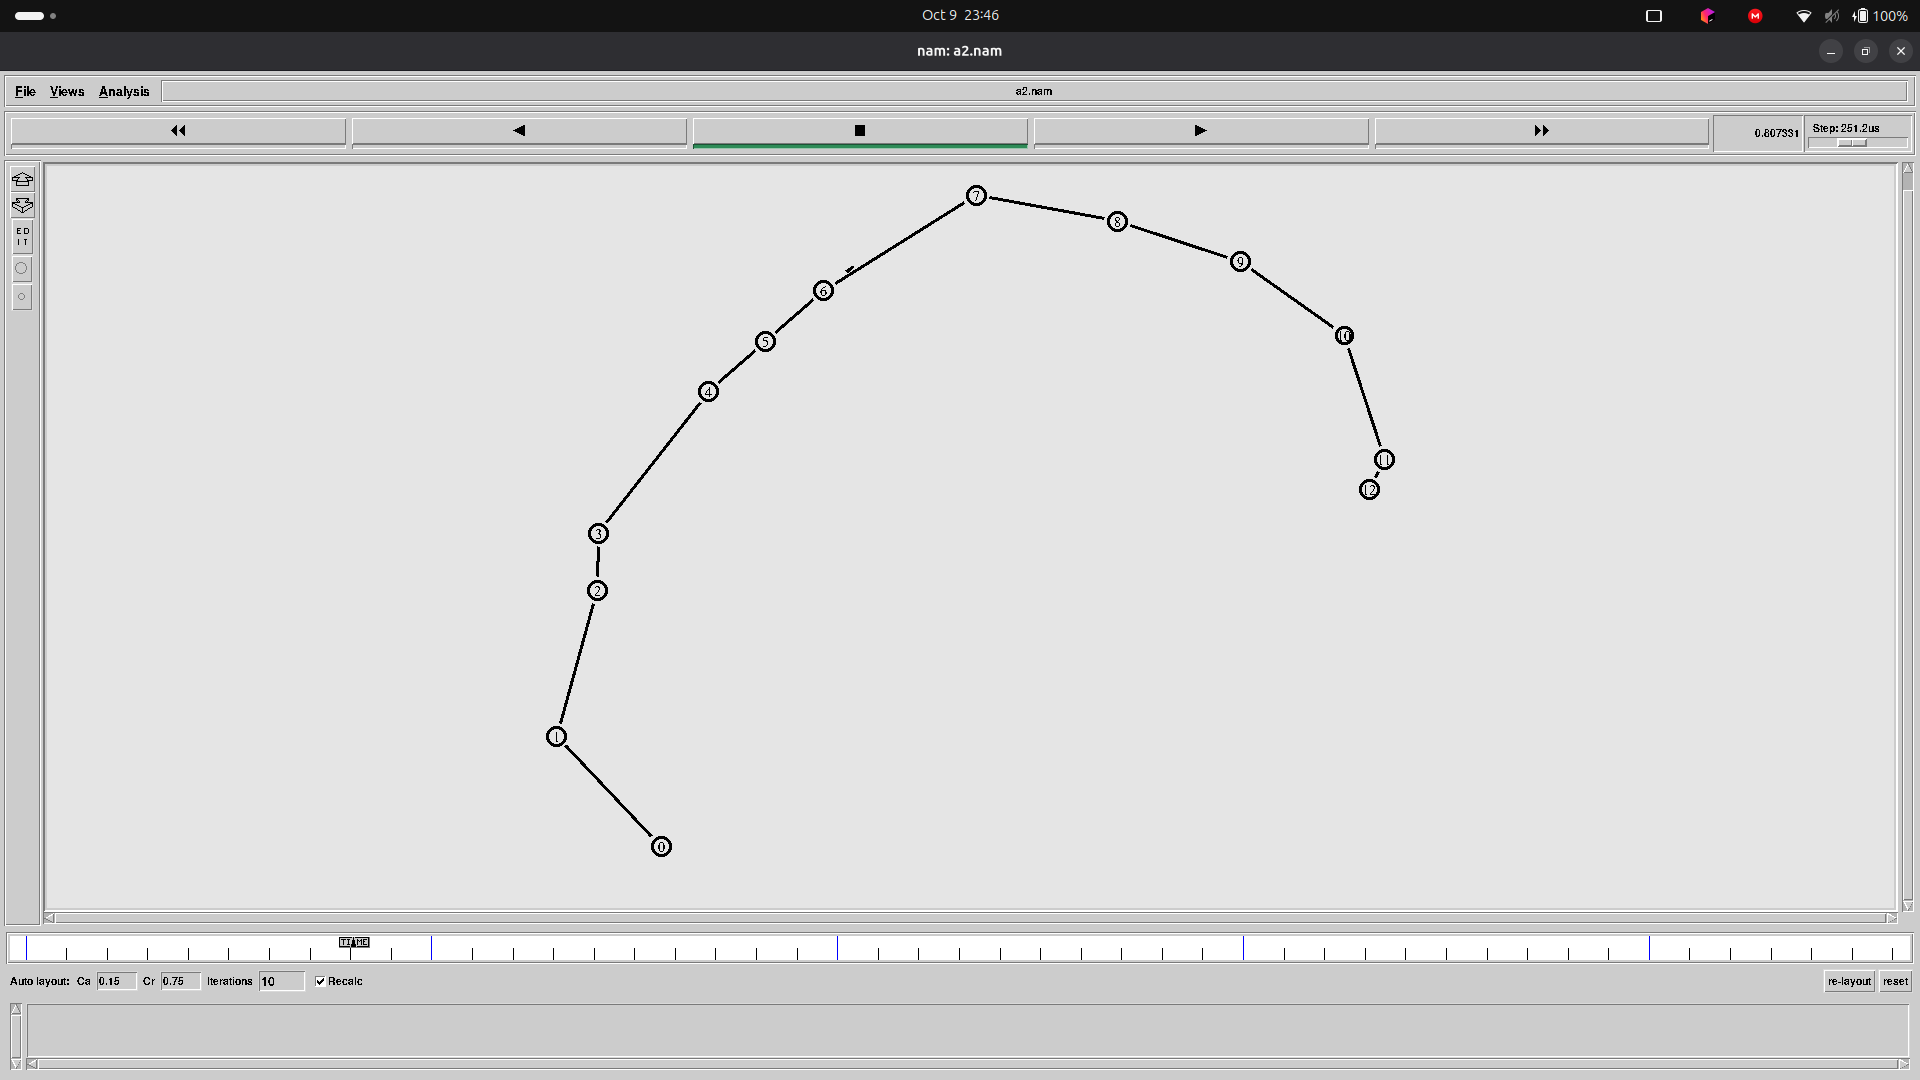
\includegraphics[width=0.85\linewidth]{nam-output.png}
		\caption{NAM simulation showing packet forwarding across traceroute path}
		\label{fig:nam}
	\end{figure}
	
	\subsection{Trace File Analysis and Discussion for First Packet}
	
	From the generated trace file (\texttt{a2.tr}) and I located the events corresponding to the first packet. These lines include the send (h), forwarding (h), and receive (r) events.
	
	\begin{adjustwidth}{-3em}{-3em}
	\begin{lstlisting}
	+ 0.5 0 1 cbr 512 ------- 0 0.0 12.0 0 0
	- 0.5 0 1 cbr 512 ------- 0 0.0 12.0 0 0
	r 0.503711 0 1 cbr 512 ------- 0 0.0 12.0 0 0
	+ 0.503711 1 2 cbr 512 ------- 0 0.0 12.0 0 0
	- 0.503711 1 2 cbr 512 ------- 0 0.0 12.0 0 0
	r 0.504972 1 2 cbr 512 ------- 0 0.0 12.0 0 0
	+ 0.504972 2 3 cbr 512 ------- 0 0.0 12.0 0 0
	- 0.504972 2 3 cbr 512 ------- 0 0.0 12.0 0 0
	r 0.505163 2 3 cbr 512 ------- 0 0.0 12.0 0 0
	+ 0.505163 3 4 cbr 512 ------- 0 0.0 12.0 0 0
	- 0.505163 3 4 cbr 512 ------- 0 0.0 12.0 0 0
	r 0.506714 3 4 cbr 512 ------- 0 0.0 12.0 0 0
	+ 0.506714 4 5 cbr 512 ------- 0 0.0 12.0 0 0
	- 0.506714 4 5 cbr 512 ------- 0 0.0 12.0 0 0
	r 0.506905 4 5 cbr 512 ------- 0 0.0 12.0 0 0
	+ 0.506905 5 6 cbr 512 ------- 0 0.0 12.0 0 0
	- 0.506905 5 6 cbr 512 ------- 0 0.0 12.0 0 0
	r 0.507096 5 6 cbr 512 ------- 0 0.0 12.0 0 0
	+ 0.507096 6 7 cbr 512 ------- 0 0.0 12.0 0 0
	- 0.507096 6 7 cbr 512 ------- 0 0.0 12.0 0 0
	r 0.508627 6 7 cbr 512 ------- 0 0.0 12.0 0 0
	+ 0.508627 7 8 cbr 512 ------- 0 0.0 12.0 0 0
	- 0.508627 7 8 cbr 512 ------- 0 0.0 12.0 0 0
	r 0.526878 7 8 cbr 512 ------- 0 0.0 12.0 0 0
	+ 0.526878 8 9 cbr 512 ------- 0 0.0 12.0 0 0
	- 0.526878 8 9 cbr 512 ------- 0 0.0 12.0 0 0
	r 0.536399 8 9 cbr 512 ------- 0 0.0 12.0 0 0
	+ 0.536399 9 10 cbr 512 ------- 0 0.0 12.0 0 0
	- 0.536399 9 10 cbr 512 ------- 0 0.0 12.0 0 0
	r 0.54261 9 10 cbr 512 ------- 0 0.0 12.0 0 0
	+ 0.54261 10 11 cbr 512 ------- 0 0.0 12.0 0 0
	- 0.54261 10 11 cbr 512 ------- 0 0.0 12.0 0 0
	+ 0.55 0 1 cbr 512 ------- 0 0.0 12.0 1 1
	- 0.55 0 1 cbr 512 ------- 0 0.0 12.0 1 1
	r 0.552551 10 11 cbr 512 ------- 0 0.0 12.0 0 0
	+ 0.552551 11 12 cbr 512 ------- 0 0.0 12.0 0 0
	- 0.552551 11 12 cbr 512 ------- 0 0.0 12.0 0 0
	r 0.552742 11 12 cbr 512 ------- 0 0.0 12.0 0 0
	\end{lstlisting}
	\end{adjustwidth}
	

	
	\begin{table}[H]
		\centering
		\begin{tabular}{|c|c|c|c|}
			\hline
			Event & Time (ms) & From$\rightarrow$To & Trace Line \\
			\hline
			Send & 0.5 & 0$\rightarrow$1 & + 0.5 0 1 cbr 512 $-------$ 0 0.0 12.0 0 0 \\
			\hline
			
			Forwarding & Multiple hops & 1$\rightarrow$2, 2$\rightarrow$3, ... 10$\rightarrow$11 & (several r, +, - lines)\\
			\hline
			
			Final Receive & 0.552742 & 11$\rightarrow$12 & r 0.552742 11 12 cbr 512 $-------$ 0 0.0 12.0 0 0 \\
			\hline
		\end{tabular}
		\caption{Trace file analysis}
		\label{tab:tf}
	\end{table}

	\begin{itemize}

	\item + = sending event at the source node
	
	\item r = receiving at each hop (including final dest)
	
	\item - = forwarding from each node
	\end{itemize}
	
		\textbf{NS2 Trace to Traceroute Relation:}
	
	\begin{table}[H]
		\centering
		\begin{tabular}{|c|c|c|}
			\hline
			Aspect & Trace File (\texttt{a2.tr}) & Traceroute Output \\
			\hline
			Number of hops & 12 total (from node 0 to 12) & 12 hops \\
			\hline
			Final destination node & \texttt{node 12} & IP: \texttt{172.67.170.169} (hop 12) \\
			\hline
			Final receiving event & \texttt{r 0.552742 11 12 ...} & Final RTT $\approx$ \texttt{48 ms} \\
			\hline
			One-way delay & $\sim$0.053 sec = \texttt{53 ms} & RTT $\approx$ \texttt{48 ms} (half RTT $\approx$ \texttt{24 ms}, but may vary due to ICMP delays) \\
			\hline
			Packet size & \texttt{512 bytes} & \texttt{60 bytes} (ICMP default) \\
			\hline
			Event pattern & \texttt{+}, \texttt{-}, \texttt{r} per hop & Echo request/reply per hop \\
			\hline
		\end{tabular}
		\caption{Comparison between Trace File and Traceroute Output}
		\label{tab:comparison}
	\end{table}
	
	
	\noindent
	\textbf{Transmission Time:}
	
	\noindent
	Packet transmission time over a 45Mbps link:
	\[
	\text{Time} = \frac{512 \times 8}{45 \times 10^6} \approx 0.09~\mathrm{ms}
	\]
	
	\noindent
	This transmission time is small but contributes to the total delay observed in the simulation. It is implicitly accounted for in NS2 during packet forwarding.
	
	
	\begin{thebibliography}{9}
		\bibitem{ookla} Speedtest by Ookla - The Global Broadband Speed Test: \url{https://www.speedtest.net/}
		\bibitem{fast} Fast.com: Internet Speed Test:
		\url{https://fast.com/}
		\bibitem{cloudflare} Internet Speed Test - Measure Network Cloudflare: \url{https://www.speedtest.net/}
		\bibitem{traceroute} Wikipedia - traceroute:
		\url{https://en.wikipedia.org/wiki/Traceroute}
		\bibitem{mark} NS2 Tutorial:
		\url{https://www.isi.edu/websites/nsnam/ns/tutorial/}
	\end{thebibliography}
	
\end{document}
